\chapter{Related work}

\section{Physics-Based Thermal Modeling Using Dymola}


Physics-based modeling is a widely adopted approach for analyzing and designing thermal management systems in electric vehicles (EVs). Dymola, which is based on the Modelica language, enables equation-oriented and acausal modeling of complex multi-domain systems. By formulating system behavior using differential-algebraic equations (DAEs), Dymola allows a physically consistent representation of thermal, fluid, mechanical, and control subsystems within a unified framework.

In EV applications, Dymola-based models are commonly used to simulate heating, ventilation, and air-conditioning (HVAC) systems for cabin climate control as well as battery thermal management systems (BTMS). These models explicitly represent key components such as the scroll compressor, condenser, evaporator, chiller, and internal heat exchanger. Each component is governed by conservation laws of mass and energy, along with thermodynamic and heat transfer relations, enabling accurate transient simulation of thermal behavior under varying operating conditions.

In this work, a Dymola model is employed to simulate the EV thermal management system, capturing both cabin HVAC operation and battery thermal regulation. The model serves as a high-fidelity representation of the real system and is parameterized by a set of operating and boundary condition inputs. In total, the model is driven by seven input parameters, summarized in Table~\ref{tab:dymola_inputs}.

\begin{table}[h!]
\centering
\caption{Dymola Model Input Parameters and Numerical Ranges}
\label{tab:dymola_input_ranges}
\renewcommand{\arraystretch}{1.3}
\begin{tabular}{|p{8cm}|p{5cm}|}
\hline
{\textbf{Parameters}} &
{\textbf{Numerical range}} \\
\hline
condenser.hxGeometry.hxHeight & 0.2 -- 0.8 (m) \\
\hline
condenser.hxGeometry.hxWidth & 0.3 -- 1.2 (m) \\
\hline
internalHX.hxGeometry.length & 0.25 -- 1 (m) \\
\hline
evaporator.hxGeometry.hxHeight & 0.2 -- 0.61 (m) \\
\hline
evaporator.hxGeometry.hxWidth & 0.11 -- 0.35 (m) \\
\hline
chiller.hxGeometry.numberOfPlates & 10 -- 15 \\
\hline
scrollCompressor.displacement & 30 -- 60 (ccm) \\
\hline
\end{tabular}
\end{table}

The simulation outputs consist of multiple time-dependent variables describing the thermal and operational behavior of the system. These include battery temperature, stored energy, vehicle velocity, and thermodynamic state variables such as pressure and enthalpy at predefined state points. An overview of the primary output parameters is provided in Table~\ref{tab:dymola_outputs}.

\begin{table}[h!]
\centering
\caption{Dymola Model Output Parameters}
\label{tab:dymola_outputs}
\begin{tabular}{|p{4cm}|p{4cm}|p{3cm}|p{4cm}|}
\hline
\textbf{Battery Temperature} &
\textbf{Stored Energy} &
\textbf{Vehicle Velocity} &
\textbf{Thermodynamic State Points} \\
\hline
Temperature vs. time (°C) &
Energy stored vs. time (Ah) &
Velocity vs. time (km/h) &
Pressure and enthalpy at state points
(\texttt{statepoint.p}, \texttt{statepoint.h}) \\
\hline
\end{tabular}
\end{table}

Each simulation is executed over a fixed duration of 30 minutes (approximately 1800 seconds), resulting in high-resolution time-series outputs. In total, the model generates 23 output variables per simulation run, each sampled at 1800 time steps. Key simulation characteristics are summarized in Table~\ref{tab:dymola_simulation}.

\begin{table}[h!]
\centering
\caption{Dymola Simulation Characteristics}
\label{tab:dymola_simulation}
\begin{tabular}{|l|l|}
\hline
\textbf{Property} & \textbf{Value} \\
\hline
Simulation duration & 30 minutes (1800 s) \\
Number of input parameters & 7 \\
Number of output variables & 23 \\
Time resolution & 1800 time steps \\
Boundary conditions & Fast Charging, Race Track \\
\hline
\end{tabular}
\end{table}

\begin{figure}[htb]\centering
        \begin{minipage}[c]{0.7\textwidth}
            \centering
            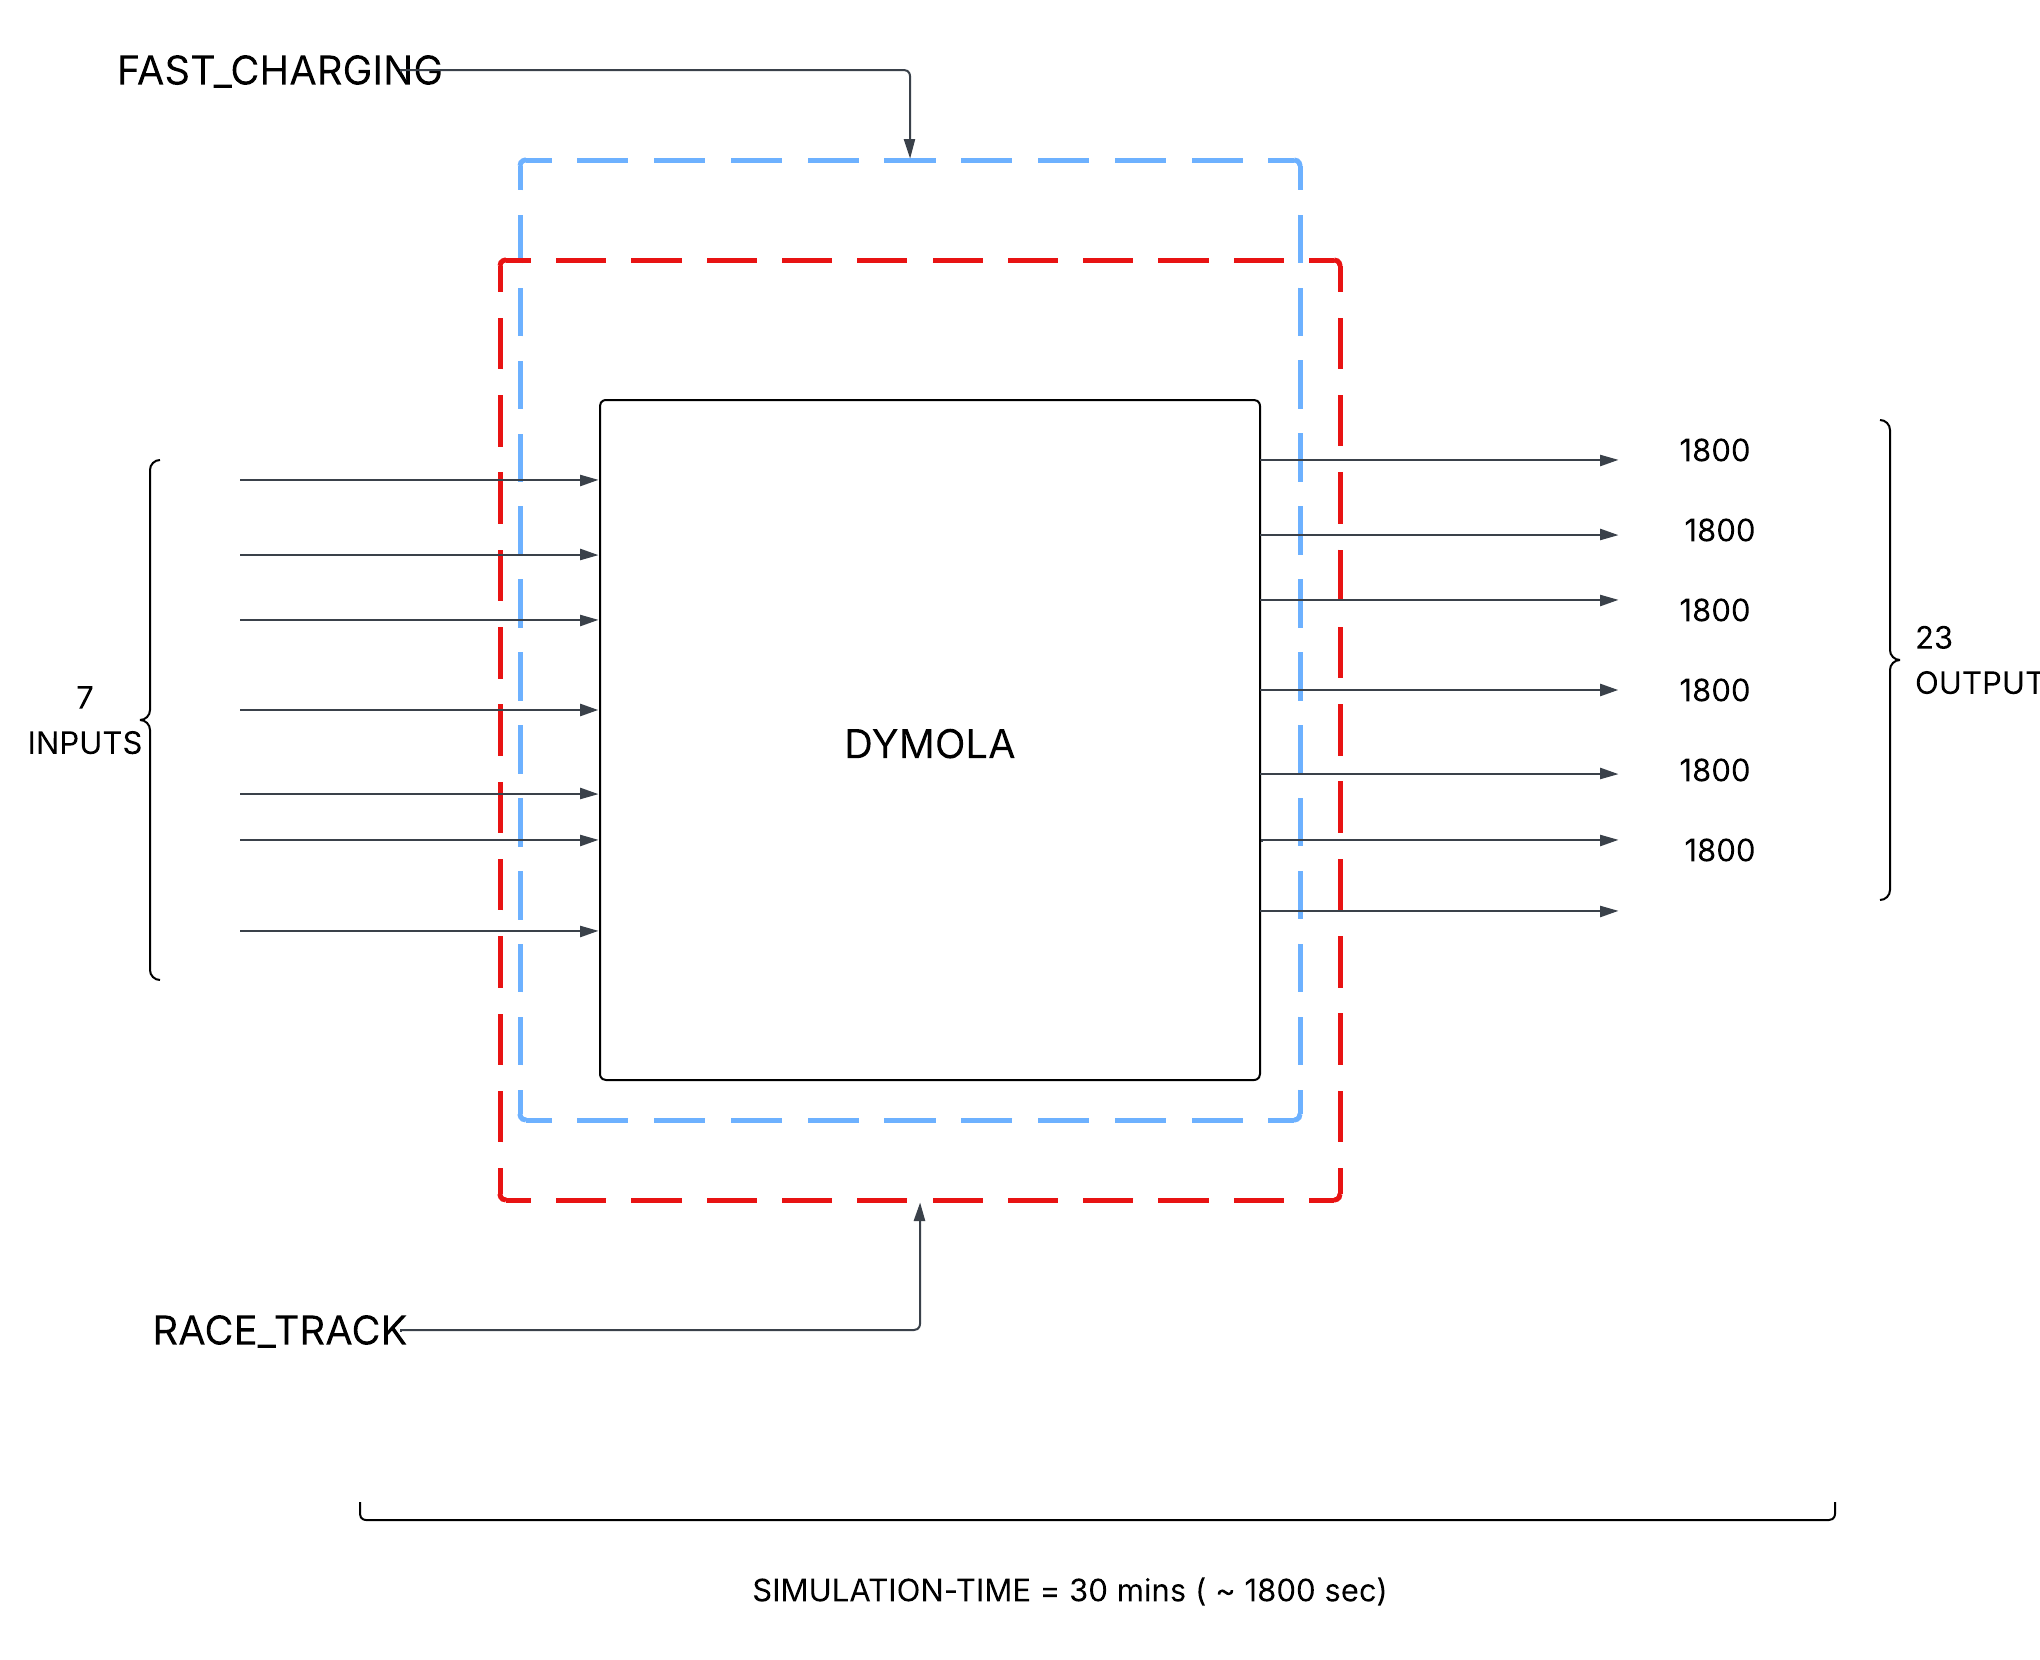
\includegraphics[width=\textwidth]{figures/Leeres Diagramm.png}
            \caption{Structure of model with Boundary Conditions.}
        \end{minipage}%
\end{figure} 

To capture representative and extreme operating regimes, simulations are conducted under two primary boundary conditions: fast charging scenarios, where the vehicle remains stationary while experiencing high thermal loads, and race-track driving conditions, characterized by sustained high power demand and aggressive thermal stress. These scenarios are commonly studied in the literature as worst-case conditions for evaluating the robustness of EV thermal management systems.

Figure~\ref{fig} illustrates the architecture of the Dymola-based EV thermal management model, highlighting the major thermal components and their interactions. Figure~\ref{fig:data_workflow} presents the overall workflow used in this thesis, where Dymola-generated simulation data are employed for training and evaluating machine learning-based surrogate models.



\begin{figure}[htb]\centering
        \begin{minipage}[c]{0.7\textwidth}
            \centering
            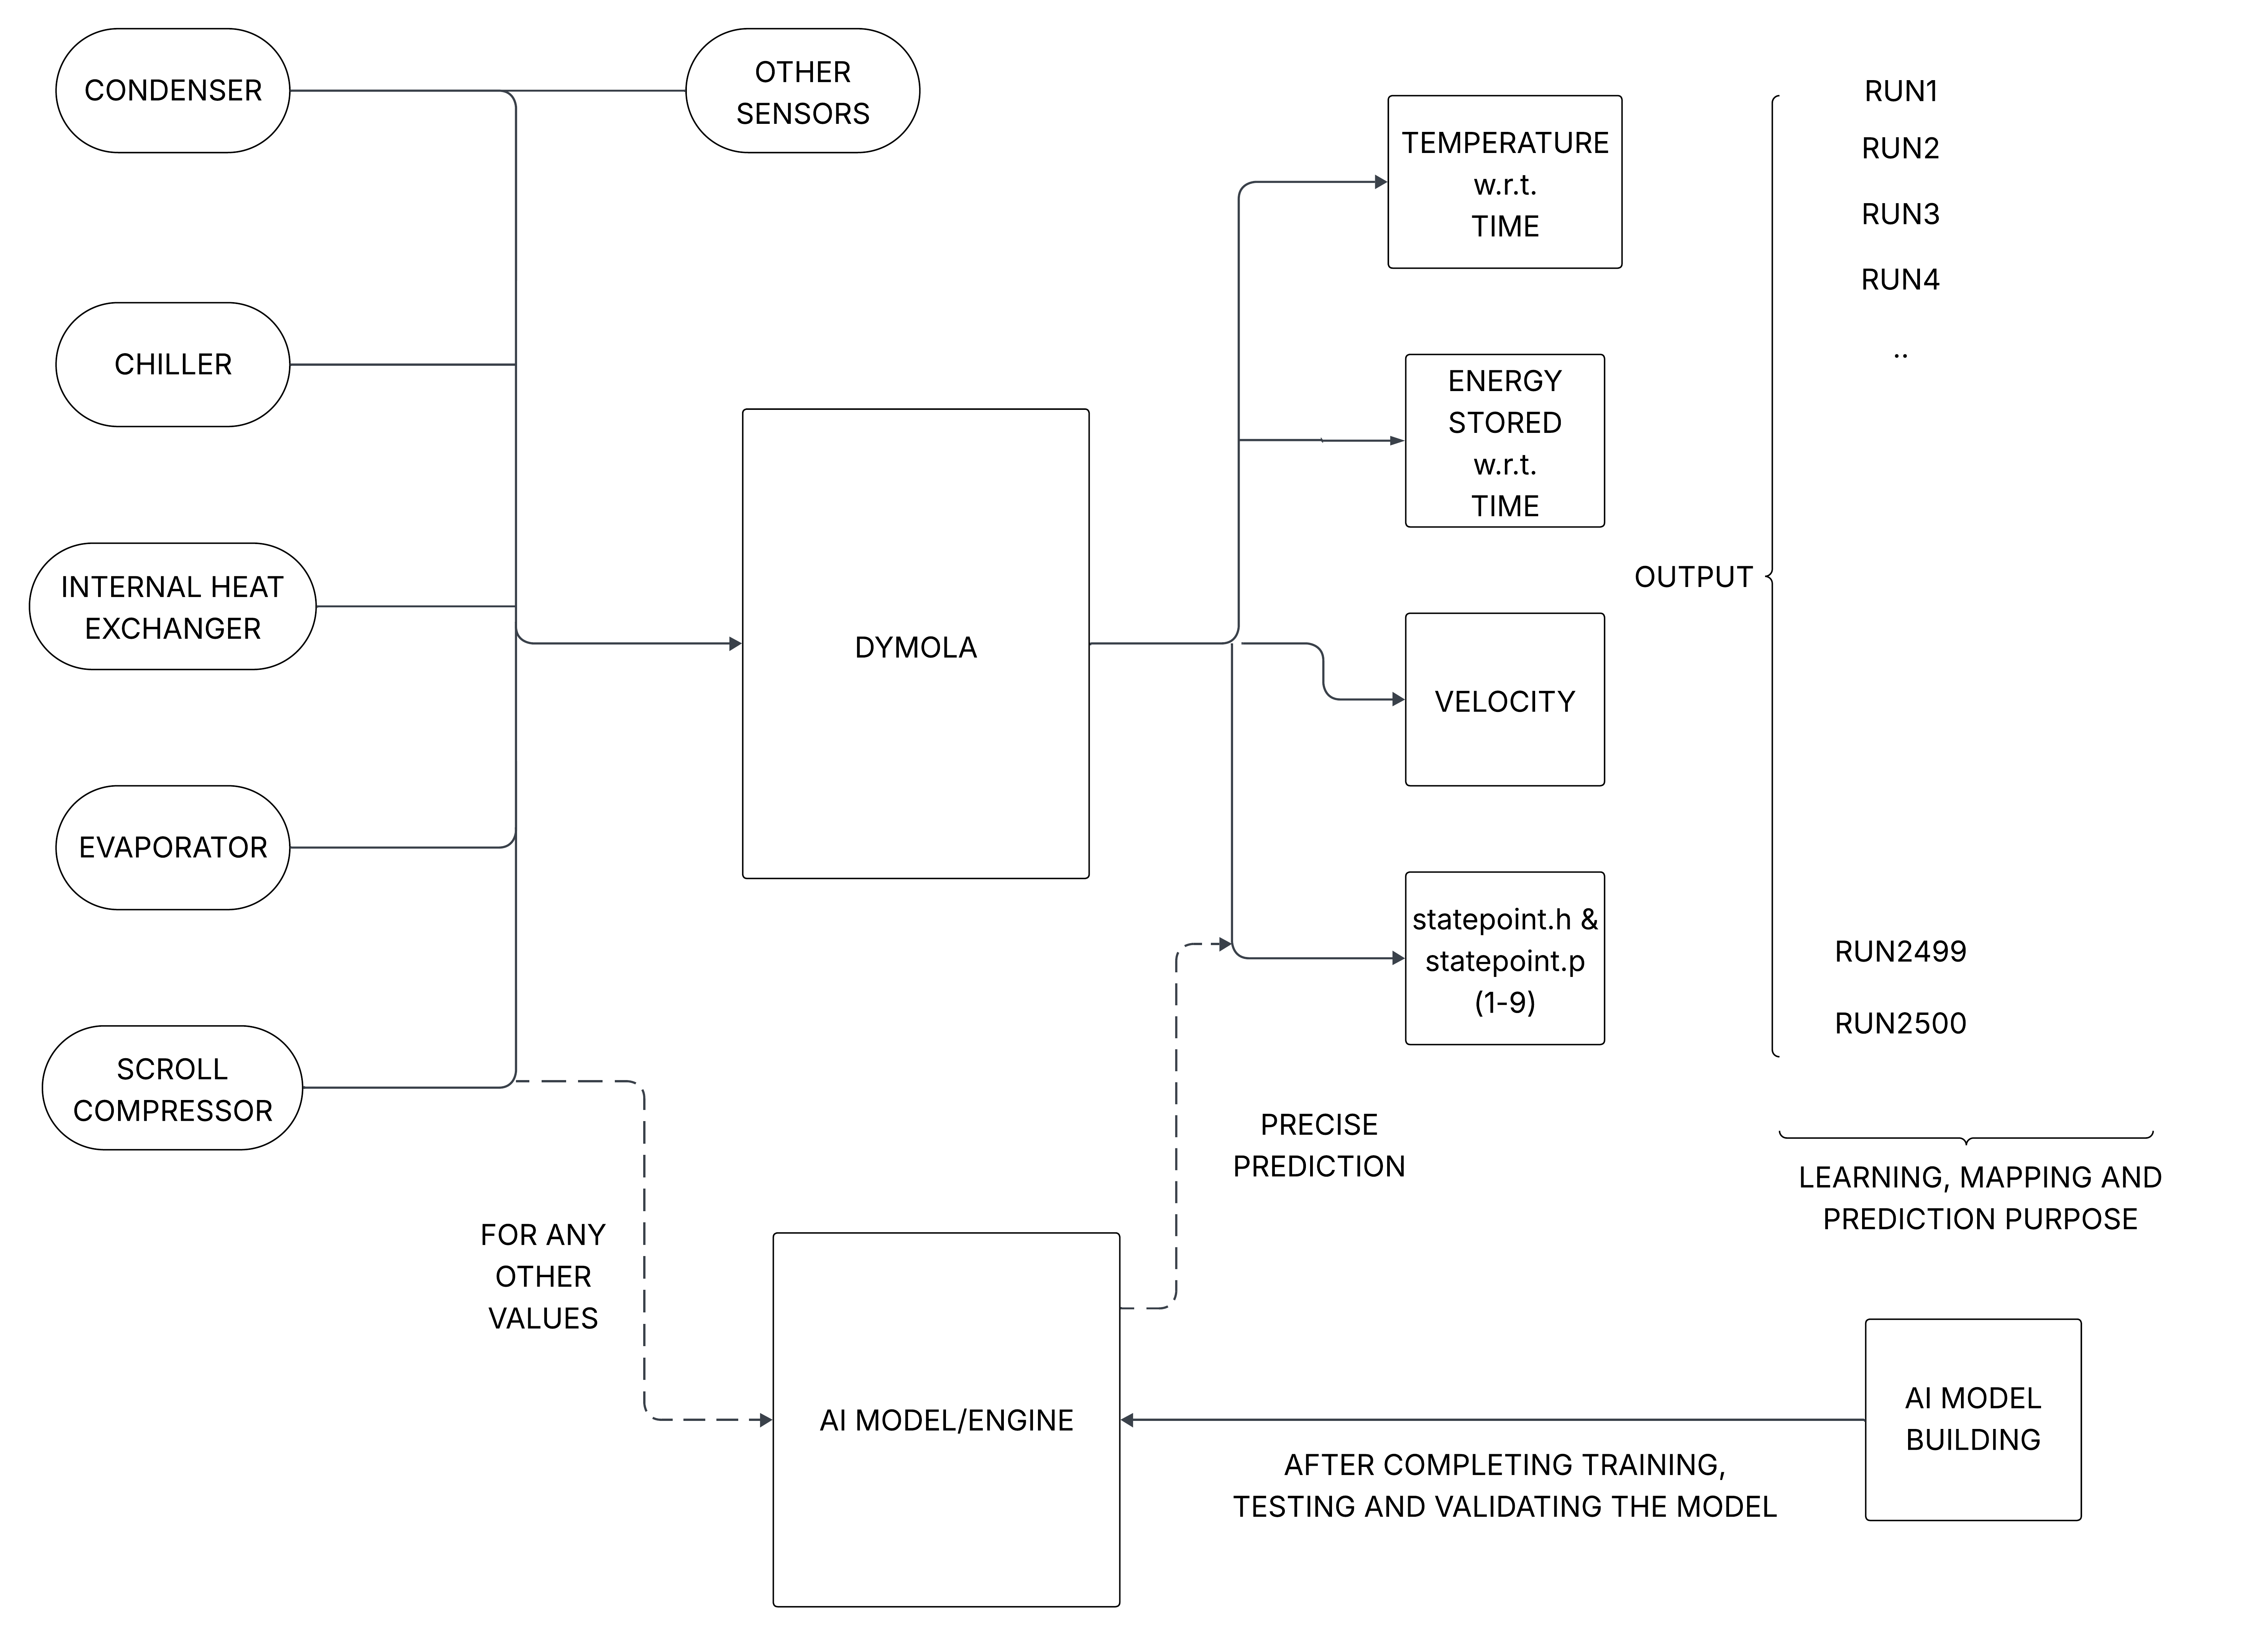
\includegraphics[width=\textwidth]{figures/Concept_Map.png}
            \caption{Workflow illustrating Dymola-based data generation and surrogate model training for fast thermal prediction.}
        \end{minipage}%
\end{figure} 



Despite their high accuracy and physical interpretability, Dymola-based simulations are computationally expensive due to the numerical integration of large-scale nonlinear DAEs. This limits their applicability for real-time control, rapid design optimization, and large-scale parameter studies. Consequently, the Dymola model in this thesis serves as a reference high-fidelity simulator for generating training data and benchmarking the performance of machine learning-based surrogate models.


\section{Latin/optimal hypercube sampling}

The generation of representative and informative training data is a critical step in the development of data-driven surrogate models for high-dimensional thermal systems. In the context of EV thermal management, the input space is defined by multiple operating and design parameters, while the corresponding outputs are high-dimensional time-series obtained from physics-based simulations. Exhaustive sampling of such input spaces using grid-based approaches quickly becomes computationally infeasible due to the curse of dimensionality.

To address this challenge, Latin Hypercube Sampling (LHS) is employed as a space-filling statistical sampling technique. LHS enables efficient exploration of high-dimensional input spaces by stratifying each input parameter range into non-overlapping intervals and ensuring that each interval is sampled exactly once. Compared to simple random sampling or full-factorial designs, LHS provides superior coverage of the input domain while requiring a significantly smaller number of samples.

In this work, LHS is applied to generate input parameter combinations for the Dymola-based EV thermal management model. The input space consists of seven independent input parameters, each defined over a prescribed numerical range based on physical and operational constraints. For a single Dymola simulation run, the generated input vector
\[
\mathbf{x} \in \mathbb{R}^{7}
\]
produces a set of time-dependent outputs
\[
\mathbf{y}(t) \in \mathbb{R}^{23}, \quad t = 1, \ldots, 1800,
\]
corresponding to 23 output variables sampled over 1800 time steps. As a result, a single simulation yields a comparatively small dataset of the form
\[
\{ 7 \; \text{inputs} \} \rightarrow \{ 23 \; \text{outputs} \times 1800 \; \text{time steps} \},
\]
which is insufficient for training robust machine learning models.

To construct a sufficiently large and diverse dataset, LHS is used to generate a total of 2050 unique input combinations. These samples are evenly distributed across two primary boundary conditions that represent extreme and practically relevant operating regimes:
\begin{itemize}
    \item \textbf{Fast Charging:} 1025 simulation runs corresponding to stationary vehicle operation under high charging currents.
    \item \textbf{Race Track:} 1025 simulation runs corresponding to high-performance driving with elevated thermal loads.
\end{itemize}

As a result, the complete dataset used for surrogate model training expands to:
\[
\{ 2050 \times 7 \; \text{inputs} \}
\;\rightarrow\;
\{ 2050 \times (23 \; \text{outputs}) \times 1800 \; \text{time steps} \}.
\]

Figure~\ref{fig:LHS} illustrates the overall data generation workflow using Optimal Hypercube Sampling. The figure highlights how the sampled input combinations are propagated through the Dymola model to generate time-series outputs under both fast charging and race-track boundary conditions.

\begin{figure}[htb]\centering
        \begin{minipage}[c]{0.6\textwidth}
            \centering
            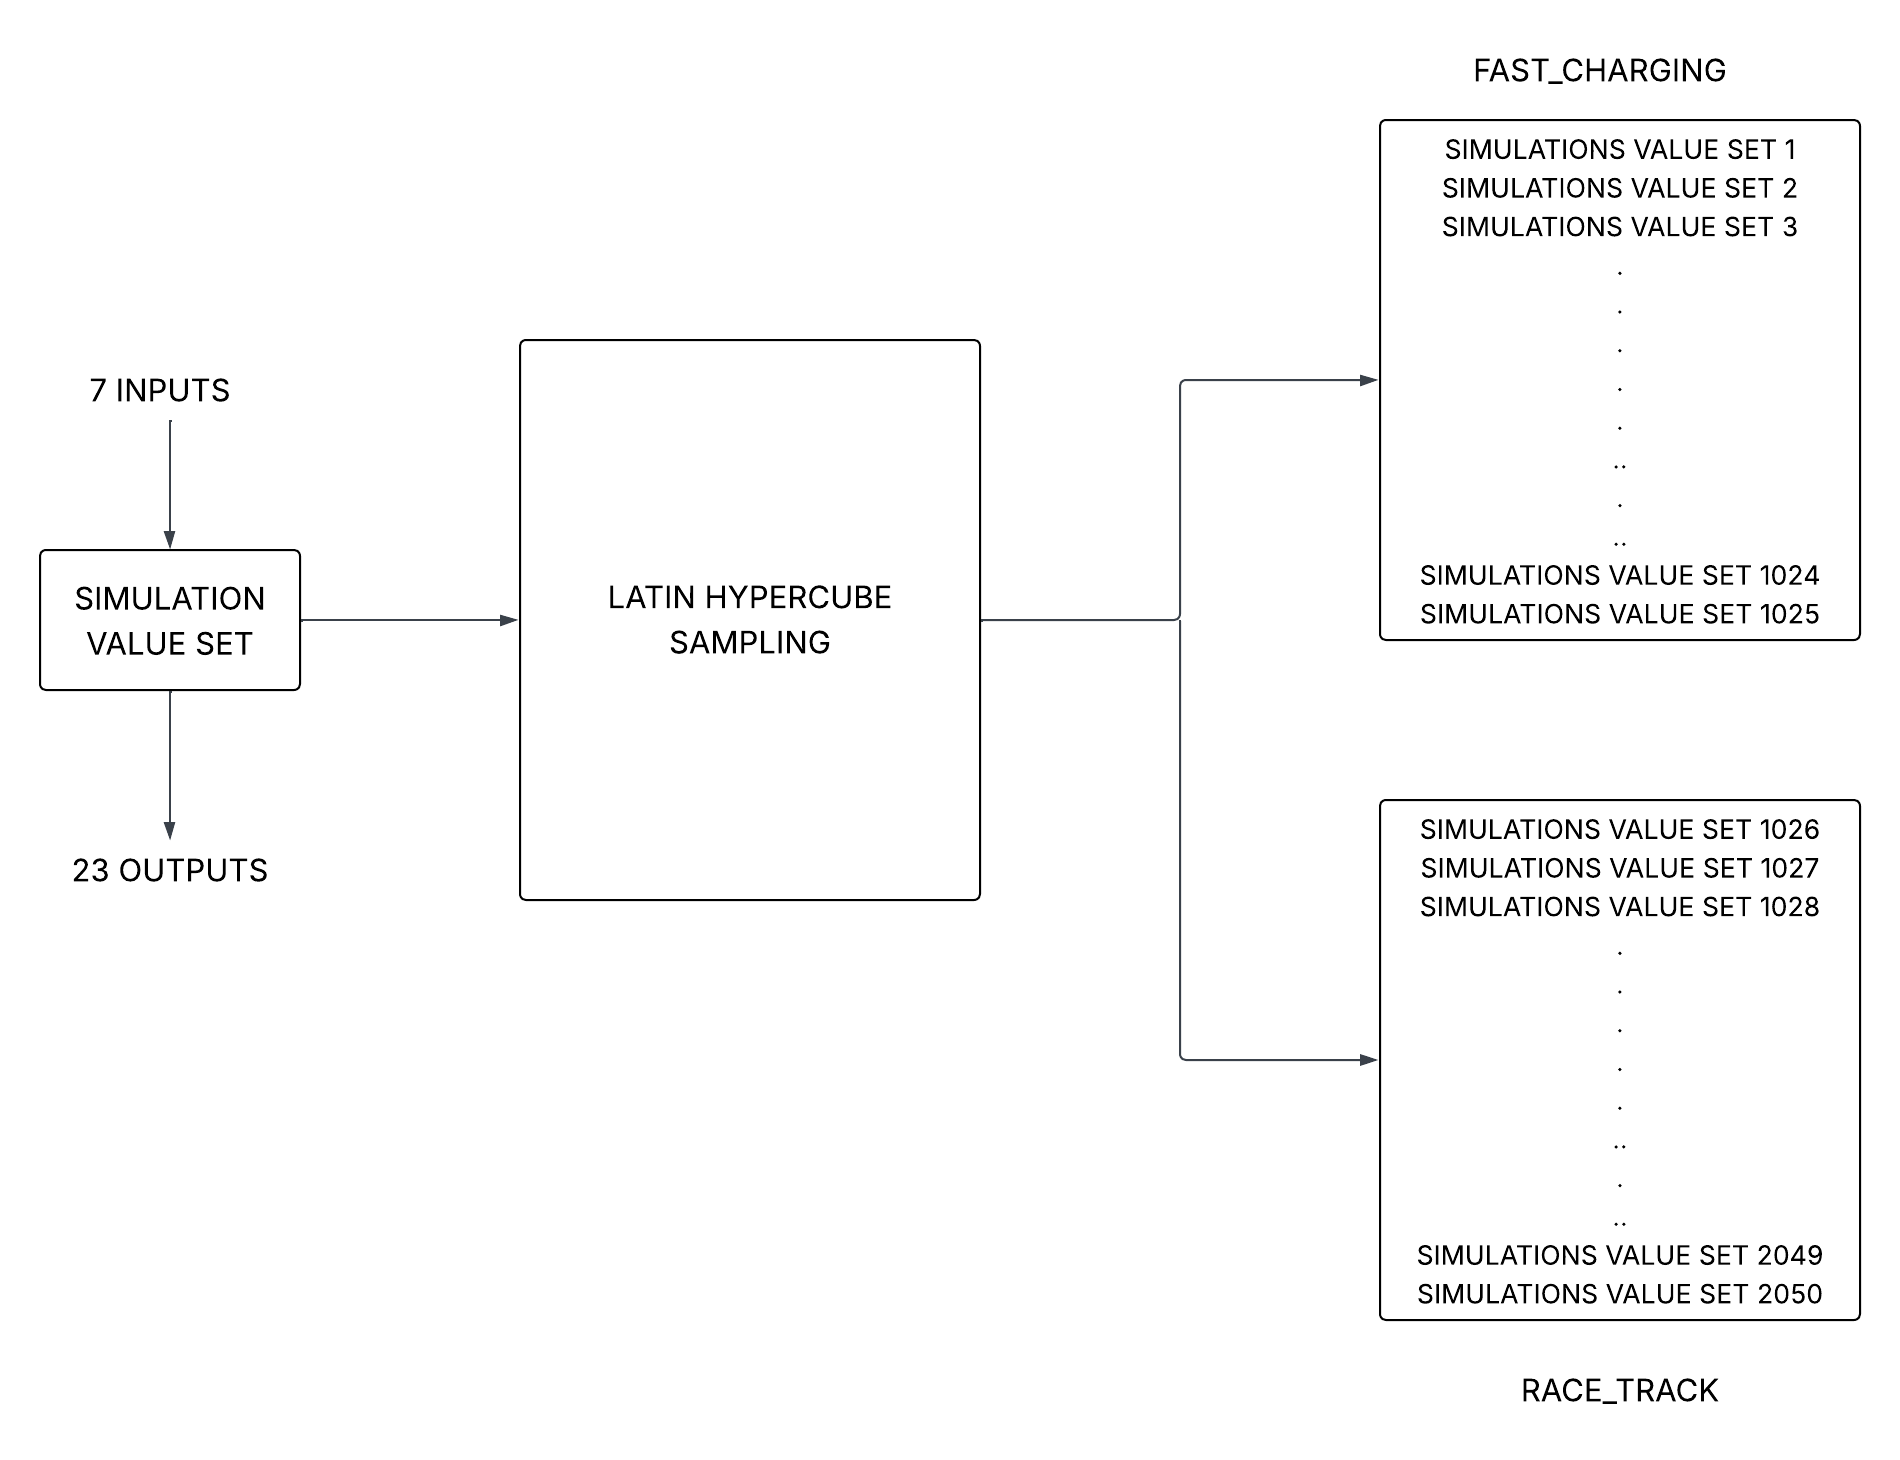
\includegraphics[width=\textwidth]{figures/LHS.png}
            \caption{Data generation workflow using Optimal Hypercube Sampling (LHS).}
            \label{fig:LHS}
        \end{minipage}%
\end{figure} 


The use of Latin Hypercube Sampling ensures a well-distributed and representative coverage of the input parameter space, which is essential for training surrogate models with strong generalization capability. By efficiently expanding the dataset while limiting the number of expensive Dymola simulations, LHS plays a key role in bridging the gap between high-fidelity physics-based modeling and data-driven learning approaches in this thesis.


\section{Principal component analysis}

Principal Component Analysis (PCA) is a statistical technique widely used for reducing the dimensionality of high-dimensional datasets while preserving the dominant variance present in the data. PCA achieves this by projecting the original data onto a smaller set of orthogonal basis vectors, referred to as principal components, which are ordered according to the amount of variance they capture.

In the context of this work, each Dymola simulation produces high-dimensional time-series outputs. Specifically, the model generates 23 output variables, each sampled over 1800 time steps, resulting in a temporal output dimension of \( 23 \times 1800 \) per simulation. Learning a direct mapping from a relatively low-dimensional input space consisting of seven input parameters to such a high-dimensional output space poses significant challenges for machine learning models, including increased computational cost, slow convergence, and poor generalization performance.

To address this issue, PCA is employed as a dimensionality reduction technique applied to the time-series outputs prior to surrogate model training. Let the time-series dataset be represented by the matrix
\[
\mathbf{X} \in \mathbb{R}^{N \times T},
\]
where \( N = 2500 \) denotes the total number of simulation runs and \( T = 1800 \) denotes the number of time steps per output variable. Each row of \( \mathbf{X} \) corresponds to a single simulation run and contains the temporal evolution of a given output signal:
\[
\mathbf{X} =
\begin{bmatrix}
x_1(t_1) & x_1(t_2) & \cdots & x_1(t_{1800}) \\
x_2(t_1) & x_2(t_2) & \cdots & x_2(t_{1800}) \\
\vdots   & \vdots   & \ddots & \vdots \\
x_N(t_1) & x_N(t_2) & \cdots & x_N(t_{1800})
\end{bmatrix}.
\]

Prior to applying PCA, the time-series data is mean-centered by subtracting the temporal mean of each feature to ensure that the principal components capture variance around the mean rather than absolute offsets. The covariance matrix of the centered data is then computed, followed by eigenvalue decomposition to obtain the principal components and their associated eigenvalues.

Only the first \( K = 5 \) principal components are retained in this work. These components collectively capture more than 99\% of the total variance of the original time-series signals, indicating a high degree of temporal redundancy in the data. As a result, the temporal representation of each output signal is reduced from
\[
1800 \;\rightarrow\; 5,
\]
while preserving the essential dynamic behavior of the system.

Applying PCA independently to each of the 23 output variables leads to a substantial reduction in the overall output dimensionality. Consequently, the structure of the dataset is transformed from:
\[
\{ 2500 \times 23 \times 1800 \}
\;\rightarrow\;
\{ 2500 \times 23 \times 5 \},
\]
where the reduced representation corresponds to a latent space defined by the retained principal components.

Figure~\ref{fig:pca_reduction} illustrates the dimensionality reduction process applied to the time-series outputs. The original high-dimensional temporal signals are projected onto a low-dimensional latent space while retaining the majority of the signal variance.

\begin{figure}[htb]
    \centering
    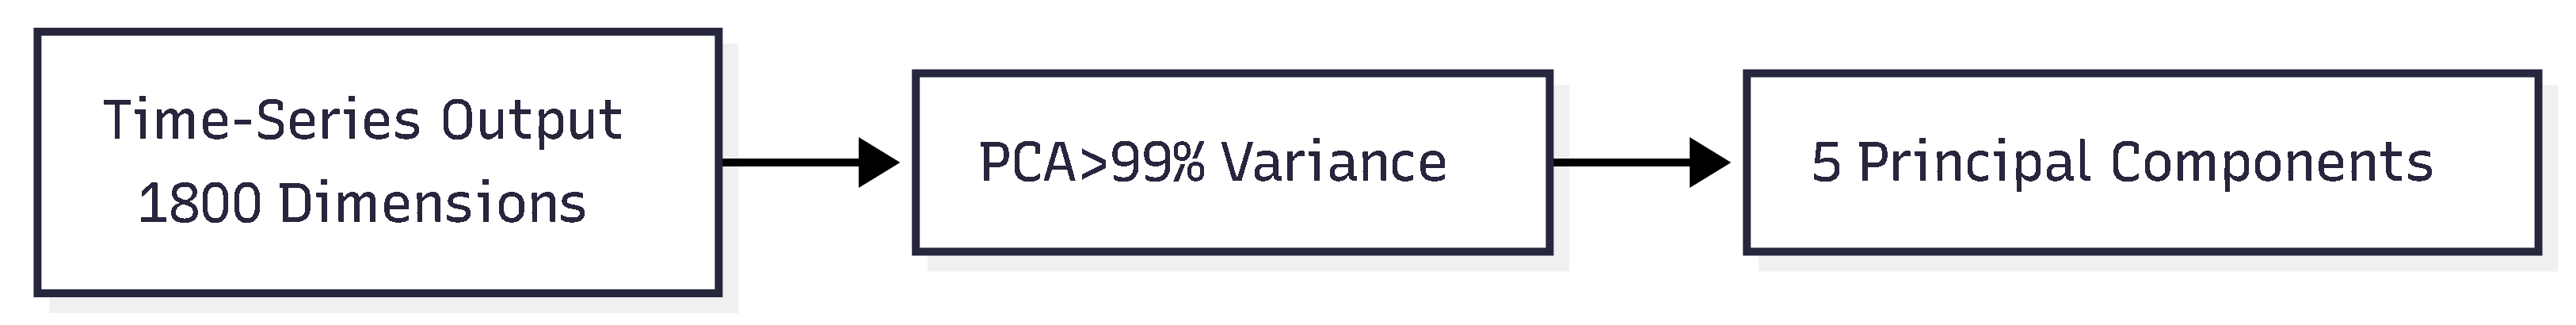
\includegraphics[width=0.9\textwidth]{figures/PCA_Time_Reduction.png}
    \caption{Dimensionality reduction of time-series outputs using PCA. The original 1800-dimensional temporal signals are projected onto a reduced set of five principal components capturing more than 99\% of the total variance.}
    \label{fig:pca_reduction}
\end{figure}

By reducing the dimensionality of the output space, PCA significantly improves the efficiency and stability of surrogate model training. The reduced latent representation enables faster learning, improved numerical conditioning, and enhanced generalization capability of machine learning models, while still allowing accurate reconstruction of the original time-series outputs through the inverse PCA transformation.
